% Cal Poly Thesis
% based on UC Thesis format
% modified by Mark Barry 2/07.
\documentclass[12pt]{ucthesis}

% Different font in captions (single-spaced, bold) ------------
\newcommand{\captionfonts}{\small\bf\ssp}

\makeatletter  % Allow the use of @ in command names
\long\def\@makecaption#1#2{%
  \vskip\abovecaptionskip
  \sbox\@tempboxa{{\captionfonts #1: #2}}%
  \ifdim \wd\@tempboxa >\hsize
    {\captionfonts #1: #2\par}
  \else
    \hbox to\hsize{\hfil\box\@tempboxa\hfil}%
  \fi
  \vskip\belowcaptionskip}
\makeatother   % Cancel the effect of \makeatletter
% ---------------------------------------

%formatting/structure based packages
   \usepackage[letterpaper]{geometry}
   \usepackage[overload]{textcase}

%packages necessary for content
   \usepackage{url}
   \usepackage{graphicx}
   \usepackage{amssymb}
   \usepackage{amsmath}
   \usepackage{algorithmicx}
   \usepackage{algpseudocode}
   \usepackage{subfig}
   \usepackage{multirow}

%paper formatting
   \setlength{\parindent}{0.25in} \setlength{\parskip}{6pt}
   \geometry{verbose,nohead,tmargin=1.25in,bmargin=1in,lmargin=1.5in,rmargin=1.3in}
   \setcounter{tocdepth}{2}

\begin{document}

% Declarations for Front Matter
\title{Aldrin's Thesis}
\author{Aldrin Montana}
\degreemonth{June}
\degreeyear{2013}
\degree{Master of Science}
\field{Computer Science}
\campus{San Luis Obispo}

\defensemonth{June}
\defenseyear{2013}

\numberofmembers{5}
   \chair{Alexander Dekhtyar, Ph.D.}
   \othermemberA{Chris Lupo, Ph.D.}
   \othermemberB{Tim Kearns, Ph.D.}
   \othermemberC{Michael Black, Ph.D.}
   \othermemberD{Eriq Augustine, Ph.D.}
\copyrightyears{seven}

\maketitle
\begin{frontmatter}
   % Custom made for Cal Poly (by Mark Barry, modified by Andrew Tsui).
   \copyrightpage

   % Custom made for Cal Poly (by Andrew Tsui).
   \committeemembershippage

   \begin{abstract}
      Pyroprinting is a novel, library-dependent microbial source
      tracking (MST) method developed by the biology department at Cal Poly,
      San Luis Obispo. This method consists of two parts: (1) sample collection
      and pyroprinting (2) comparison of produced pyroprints against a
      database. Cal Poly Library of Pyroprints (CPLOP) is a web-based database
      application that provides storage and analysis of pyroprints. CPLOP
      currently contains 4500 pyroprints and is growing rapidly as students and
      researchers continue adding data. Hierarchical clustering, the
      traditional method of analysis used by biologists, is inadequate. While
      the clusters it produces are acceptable, pyroprinting requires a new
      method of analysis that is both scalable and flexible. Hierarchical
      clustering falls short in these regards as it is unable to efficiently
      cluster new data with already clustered data and it is incapable of
      utilizing available metadata. We propose ontology-based hierarchical
      clustering (\textit{OHClust!}), a modification of hierarchical clustering
      that uses an ontology to direct the order in which data is clustered. In
      this paper we discuss the strengths and weaknesses of OHClustering and
      analyze its performance in comparison to hierarchical clustering.
   \end{abstract}

   \begin{acknowledgements}
      This work was supported in part by an undergraduate education grant from
      the W.M. Keck foundation.
   \end{acknowledgements}

   \tableofcontents

   \listoftables
   \listoffigures
\end{frontmatter}

\pagestyle{plain}

\renewcommand{\baselinestretch}{1.66}

%%%%%%%%%%%%%%%%%%%%%%%%%%%%%%%%%%%%%%%%%%%%%%%%%%%%%%%%%%%%%%%%%%%%%%%%%%%%%%%
%%%%%%%%%%%%%% ----------------- Main chapters ---------------------- %%%%%%%%%
%%%%%%%%%%%%%%%%%%%%%%%%%%%%%%%%%%%%%%%%%%%%%%%%%%%%%%%%%%%%%%%%%%%%%%%%%%%%%%%

\chapter{Introduction}\label{chap:intro}
   To maintain the cleanliness of current ``fishable and swimmable'' bodies of
   water, and improve the cleanliness of others, health and environmental
   protection agencies have been interested in the ability to track sources of
   fecal contamination at the species level~\cite{Scott:CurrentMST,
   Simpson:StateOf, Desmarais:SoilInfluence}. Investigating fecal contamination
   is especially necessary in waters used for human recreation where dangerous
   pathogens are transferable. Further, relating a fecal contamination back to
   a particular species is an important first step in controlling fecal
   contamination and managing bacterial risks by enabling natural resource
   managers to address fecal contamination at its source.

   Within the last decade, several techniques of identifying and descriminating
   between various sources of fecal bacteria in an environment have been
   studied and developed~\cite{Sargeant:ReviewMST, Hagedorn:MST_TMDL,
   Lowe:FocusMST, Rivera:MSTCharacterization, Cornelison:MSTTools,
   Chase:FloridaMST}. This field of study, \textit{Microbial source tracking}
   (MST) dates back to the 1960s with the use of fecal coliform-to-fecal
   streptococci ratios. Many MST techniques rely on the genotypic or
   phenotypic analyses of fecal indicator bacteria (FIB) such as fecal
   coliforms, fecal enterococci, or \textit{Escherichia coli} (\textit{E.
   coli}). FIB are bacteria that are found in the intestinal tracts of various
   host animals and, when found, can be used to indicate or approximate the
   level of fecal contamination in water~\cite{Simpson:StateOf}. In 1999, the
   first review of MST techniques was published by Debby
   Sargeant~\cite{Sargeant:Methods}, followed by another review in November
   2011~\cite{Sargeant:ReviewMST}. In her 2011 review of current MST methods,
   she describes the MST field as a new, experimental field that has been
   continuously studying and developing new methods over several
   years~\cite{Sargeant:ReviewMST}. Fortunately, there have been publications
   that provide notable overviews of MST techniques and
   applications~\cite{Hagedorn:CaseStudies, Domingo:Current,
   Harwood:RapidMethods} within the last couple of years. Despite the highly
   experimental nature of MST at this phase of its development, Sargeant claims
   that there is strong pressure on natural resource managers to use these
   techniques to identify bacterial sources of
   pollution~\cite{Sargeant:ReviewMST}.

   The work described in this paper addresses the comparison of fingerprints of
   bacterial isolates for a library-dependent MST technique developed by the
   Cal Poly Biology department. As described by Sargeant, the library used by a
   library-dependent MST technique is a database of fingerprints from
   individual bacterial isolates, obtained from potential sources of fecal
   contamination. This library allows for the storage and retrieval of
   bacterial fingerprints to identify and differentiate between bacterial
   \textit{strains}--groups of bacterial isolates that have similar genotypes.
   Bacterial isolates are considered part of the same strain if their
   fingerprints are determined to be similar. Determining the source of a fecal
   contamination relies on building an appropriately sized library. Once an
   appropriately sized library has been built, it is then possible to associate
   a bacterial isolate to the host species with which its determined bacterial
   strain has previously been associated. Although not conclusively
   established, this type of MST technique relies on the relationship between
   bacterial strains and various host species. For instance, there are many
   different kinds of \textit{E. coli}, some of which are only present in
   humans, while others are only found in other species or particular regions
   of the world. In this way, the library must be populated with bacterial
   isolates collected from known species so that relationships between
   bacterial strains and host species can emerge. Additionally, the selection
   of an appropriate FIB is important and will affect interpretations of
   analyses differently. Unfortunately, since the definition of a bacterial
   strain is fuzzy and dependent on the research group and research task at
   hand, the level of similarity required for two organisms be considered part
   of the same strain is defined and established differently from research
   group to research group.

   Interestingly, Sargeant claims that the MST field is moving away from
   library-dependent methods and towards library-independent methods. While
   the discussion of this topic is outside the scope of this thesis, it's
   worthwhile to mention that the reason for this is that library-dependent
   methods require a significant effort to build an appropriately large, useful
   library. The library also needs to include fingerprints relative to the
   environment being investigated. However, it is currently a more reliable,
   flexible MST technique that allows for the identification of hosts beyond
   humans and some domestic animal species.

   Generally, library-dependent methods being developed have shifted
   significantly towards genotypic analysis of collected bacteria and away from
   phenotypic analysis. Genotypic analysis strives to separate observed
   bacterial samples by differentiating between bacteral strains based on
   fingerprints of the bacterial genome. When compared to phenotypic methods,
   genotypic methods are advantageous since they use differences in nucleic
   acids to distinguish between strains of \textit{E. coli} with greater
   sensitivity~\cite{Anderson:Diversity, Gordon:StrainTyping, Ochman:Enzyme,
   Scott:CurrentMST, Simpson:StateOf}.

\chapter{Background}\label{chap:background}
   %TODO include references for posters and other published material
   To address some of the common complaints regarding other methods of strain
   differentiation, the Biology department at Cal Poly, San Luis Obispo has
   been developing a genotypic, library-dependent MST method,
   \textit{pyroprinting}. Current genotypic methods can be labor intensive or
   financially expensive, and many have issues in reproducibility when
   identifying known \textit{E. coli} strains~\cite{Gordon:StrainTyping,
   Scott:CurrentMST, Simpson:StateOf}. This is especially evident in
   longitudinal single-host studies of microbial strains, which are a key
   problem for MST studies~\cite{Simpson:StateOf, Anderson:Diversity,
   Schlager:Clonal}. In these studies, bacterial cultures are typically grown
   from samples collected in roughly even intervals (daily, weekly, etc.) from
   a single individual. These studies are concerned with the total number of
   strains of a particular bacterium (e.g. \textit{E. coli}) present in a host
   at a given moment in time, strain turnover over time, the presence of
   dominant strains, change of strain dominance over time, as well as
   corresponding cause-and-effect questions (i.e. what causes all these
   changes)~\cite{Anderson:Diversity, Caugant:Diverse, Sears:Persist,
   Simpson:StateOf}.
   
   Several students in the Biology department have conducted research projects
   focusing on the use and applicability of pyroprinting. Among the various
   research projects, one student has established and piloted a novel framework
   for genotypic microbial analysis of bacteria (so far \textit{E. coli} only)
   in longitudinal studies~\cite{Montana:ChronoCluster, Montana:CRC}. This
   framework incorporates \textit{pyroprinting} and an \textit{in-silico}
   source strain differentiation method based on a clustering algorithm further
   described in Section \ref{sec:ohclust}.
   
   The work presented in this paper is the computational analysis which
   determines what bacterial isolates are of the same strain. More
   specifically, this paper compares the use of two clustering
   algorithms--Hierarchical Agglomerative Clustering and OHClust!--in order to
   characterize and better understand the performance, effects of parameter
   tuning, and results of OHClust! for pyroprinting. This paper also goes on to
   describe how OHClust! can be useful when applied to other types of data. The
   rest of this chapter fully explains the context of this work as well as
   establishes terminology that will be used throughout the rest of this
   paper.

   \section{Bacterial Sampling and Data Collection}\label{sec:sampling}
      The process of sampling begins with the selection of stool. From the
      stool, $N$ samples are collected, isolated, and cultured in preparation
      for polymerase chain reaction (PCR) and eventually pyroprinting. Each of
      the bacterial samples are then streaked onto MacConkey agar plates for
      single isolated colonies (isolate for short) and grown overnight.
      Isolates are confirmed for the target bacteria at the end of the process.
      Any isolates that are not of the target bacteria are left unused. This
      process is highlighted in a previous submission to the CSU research
      competition~\cite{Montana:CRC} which describes a study where \textit{E.
      coli} was sampled once a month for six months from three individuals--two
      females and one male--ranging in age from $20-25$.
      
   %TODO this section suckss
   \section{Strains}\label{sec:strains}
      The objective of microbial source tracking is to be able to relate the
      source--host species--of a fecal contamination so that water treatment
      can be approached by addressing the source of the problem instead of
      reactively treating the problem. Pyroprinting does this by creating
      a fingerprint of bacterial isolates, storing this fingerprint and
      associated metadata in a library, and then comparing fingerprints of
      isolates in the wild to known isolates in the library. Naturally, the
      library is a database, and to determine similar, or highly-related,
      isolates we use clustering. Each cluster that a clustering algorithm
      produces corresponds to an observable strain of bacteria.

   \section{Pyroprinting}\label{sec:pyroprinting}
      Pyrosequencing is a DNA sequencing process where a new strand of DNA,
      which we will refer to as the \textit{sequencing strand}, is built
      incrementally, complementary to the strand of DNA being sequenced, which
      we will call the \textit{template strand}. Ronaghi, et al. describe the
      pyrosequencing process in more detail~\cite{ronaghi:shedsLight}. This
      process takes place on a \textit{plate} containing many
      \textit{wells}--$24$ wells for the \textbf{PyroMark Q24}, a
      pyrosequencing machine manufactured by Qiagen. A pyrosequencing
      \textit{run} denotes the entirety of the pyrosequencing process for a
      single plate. While only one plate can be processed per run, each well on
      the plate contains a separate pyrosequencing reaction. For the PyroMark
      Q24, this means that a single run can pyrosequence 24 separate template
      strands. During a run, nucleotides--\textbf{A}denine, \textbf{T}hymine,
      \textbf{C}ytosine, or \textbf{G}uanine--are dispensed into each well of
      the plate.
      
      The order in which nucleotides are dispensed is determined by
      a parameter called the \textit{dispensation sequence}. The dispensed
      nucleotide binds with the next available unbound nucleotide of the
      template strand if they are complementary--\textbf{A} binds with
      \textbf{T} and \textbf{C} binds with \textbf{G}. If the dispensed
      nucleotide binds to the template strand, the sequencing strand is
      extended and light is emitted. The observed light emittance is
      proportional to the amount of nucleotides incorporated into the
      sequencing strand. For example, if \textbf{A} is incorporated into the
      sequencing strand and the light emittance is measured at 100, then
      \textbf{T} is incorporated into the sequencing strand with light
      emittance 200, then the template strand has twice as many \textbf{T}
      nucleotides proceeding a series of \textbf{A} nucleotides. Any remaining
      nucleotide not incorporated is enzymatically destroyed and the next
      nucleotide in the dispensation sequence is dispensed.
      
      The pyrosequencing machine measures and records the light emitted from
      the binding reaction to construct a \textit{pyrogram} of the template DNA
      strand. A pyrogram is a graph that plots light emittance of DNA synthesis
      reactions with the dispensed nucleotide, depicted in Figure
      \ref{fig:pyrogram}. Modern pyrosequencing equipment allows for
      dispensation sequences of up to 200 nucleotides in length, however, the
      quality of the sequencing process deteriorates beyond 100--120
      dispensations.

      Pyrosequencing is a relatively cheap and quick DNA sequencing method.
      That is to say, it is not as cheap and powerful as modern DNA sequencing
      processes known as ``Next Generation Sequencing'' (NGS), but it is one of
      the cheapest and quickest of non-NGS sequencing processes. While
      pyrosequencing is cheap compared to other academically accessible DNA
      sequencing processes, sequencing a strand of DNA in 100--200 nucleotide
      chunks for strain differentiation purposes becomes expensive very
      quickly. To adapt pyrosequencing for strain differentiation purposes, the
      Biology department decided to pyrosequence multiple strands of DNA in
      parallel in a well. This process, referred to as \textit{pyroprinting},
      leverages the fact that introduced nucleotides will bind with the first
      available nucleotide of the template strand by sequencing multiple
      template strands in the same reaction. This already takes place in the
      case where the template strands are identical (DNA amplification), but
      the template strands used in pyroprinting are not necessarily identical.

      Pyroprinting generates pyroprints (DNA fingerprints) based on the DNA
      from two highly variable regions of the microbial genome. These regions,
      called \textit{intergenic transcribed spacers} (ITS), are regions of the
      genome located between two genes that contains non-coding DNA. For
      microbial source tracking, the 16S--23S ITS region, located between the
      16S and 23S genes, is a widely accepted ITS region for comparing
      strains~\cite{Boyer:ITS, Roth:Phylo, Tyler:Primers}. Also mentioned in
      this paper is the 23S--5S ITS region. Both of these regions of DNA are
      non-coding, and thus are able to accumulate more variability, or
      mutations, than regions of DNA that code for important proteins or RNAs
      due to lack of selective pressures. This variability manifests in
      nucleotide changes in the genome, thus while the DNA of the 16S, 23S, and
      5S genes are conserved, the same is not necessarily true for the ITS
      region between them. However, these regions may be more or less useful
      depending on the choice of FIB.
      
      The use of the 16S--23S and 23S--5S ITS regions are especially important
      for the work described in this paper because the microbial genome has
      \textit{several copies} of each ITS region. The \textit{E. coli} genome,
      specifically, has seven replicates of both the 16S--23S and 23S--5S ITS
      regions~\cite{Boyer:ITS, Roth:Phylo, Tyler:Primers}. Pyroprinting relies
      on the use of each replicate of the target ITS region that exists in the
      microbial genome. That is, for a single microbial isolate, each copy of
      the 16S--23S ITS region is pyrosequenced together, and each copy of the
      23S--5S ITS region is pyrosequenced together. Thus, for a microbial
      isolate, two \textit{pyroprints} are constructed such that each pyroprint is
      an aggregate of several, possibly different, template strands. Operating
      under the assumption that the variability between ITS regions of the
      genome will vary for different strains of \textit{E. coli}, a pyroprint
      acts as a DNA fingerprint for each strain--a pyrogram fingerprint.
      
      The algorithm, discussed in Chapter \ref{chap:algorithm}, is flexible
      enough to address any number of regions and any regions used, and the
      implementation, discussed in Chapter \ref{chap:implementation} discusses
      how this is handled in practice.

      \begin{figure}[t]
      \centering
      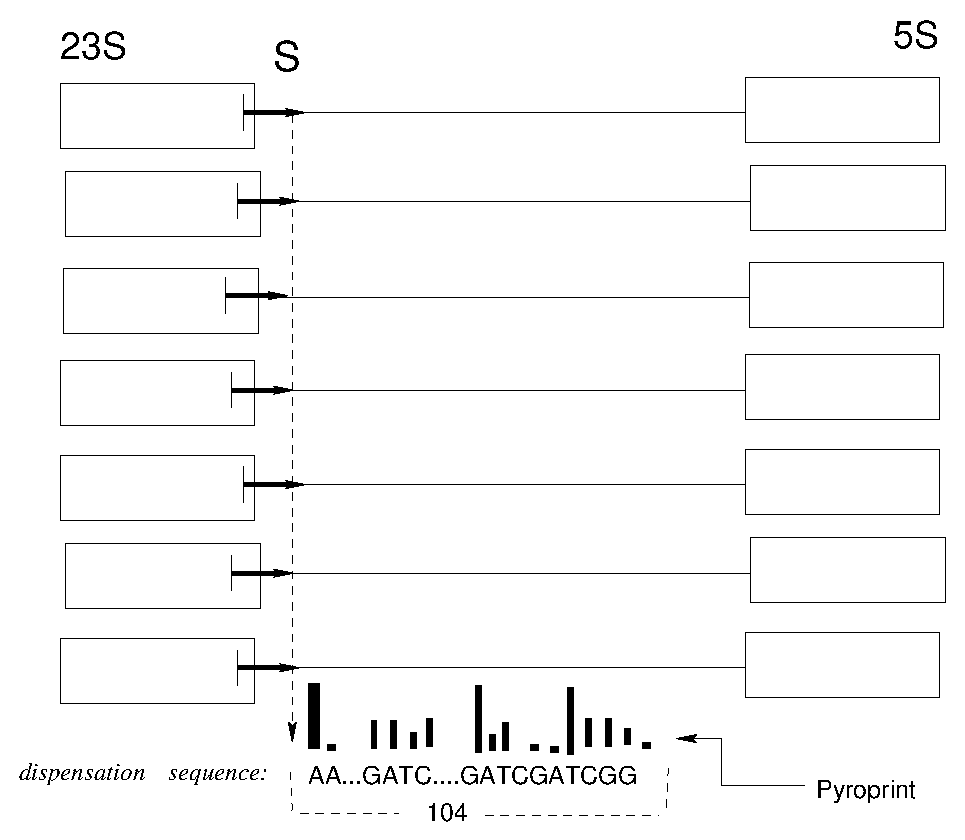
\includegraphics[width=\columnwidth]{graphics/pyroprinting.eps}
      \caption{Pyroprinting process: light intensities (black bars at the
               bottom) are observed for each nucleotide in the dispensation
               sequence. Open boxes represent conserved DNA sequences in the
               23S and 5S rRNA genes and \textnormal{S} indicates the point at
               which the sequencing primer binds to the DNA, beginning the
               sequencing process.}
      \label{fig:pyroprinting}
      \end{figure}

      \begin{figure}[t]
      \centering
      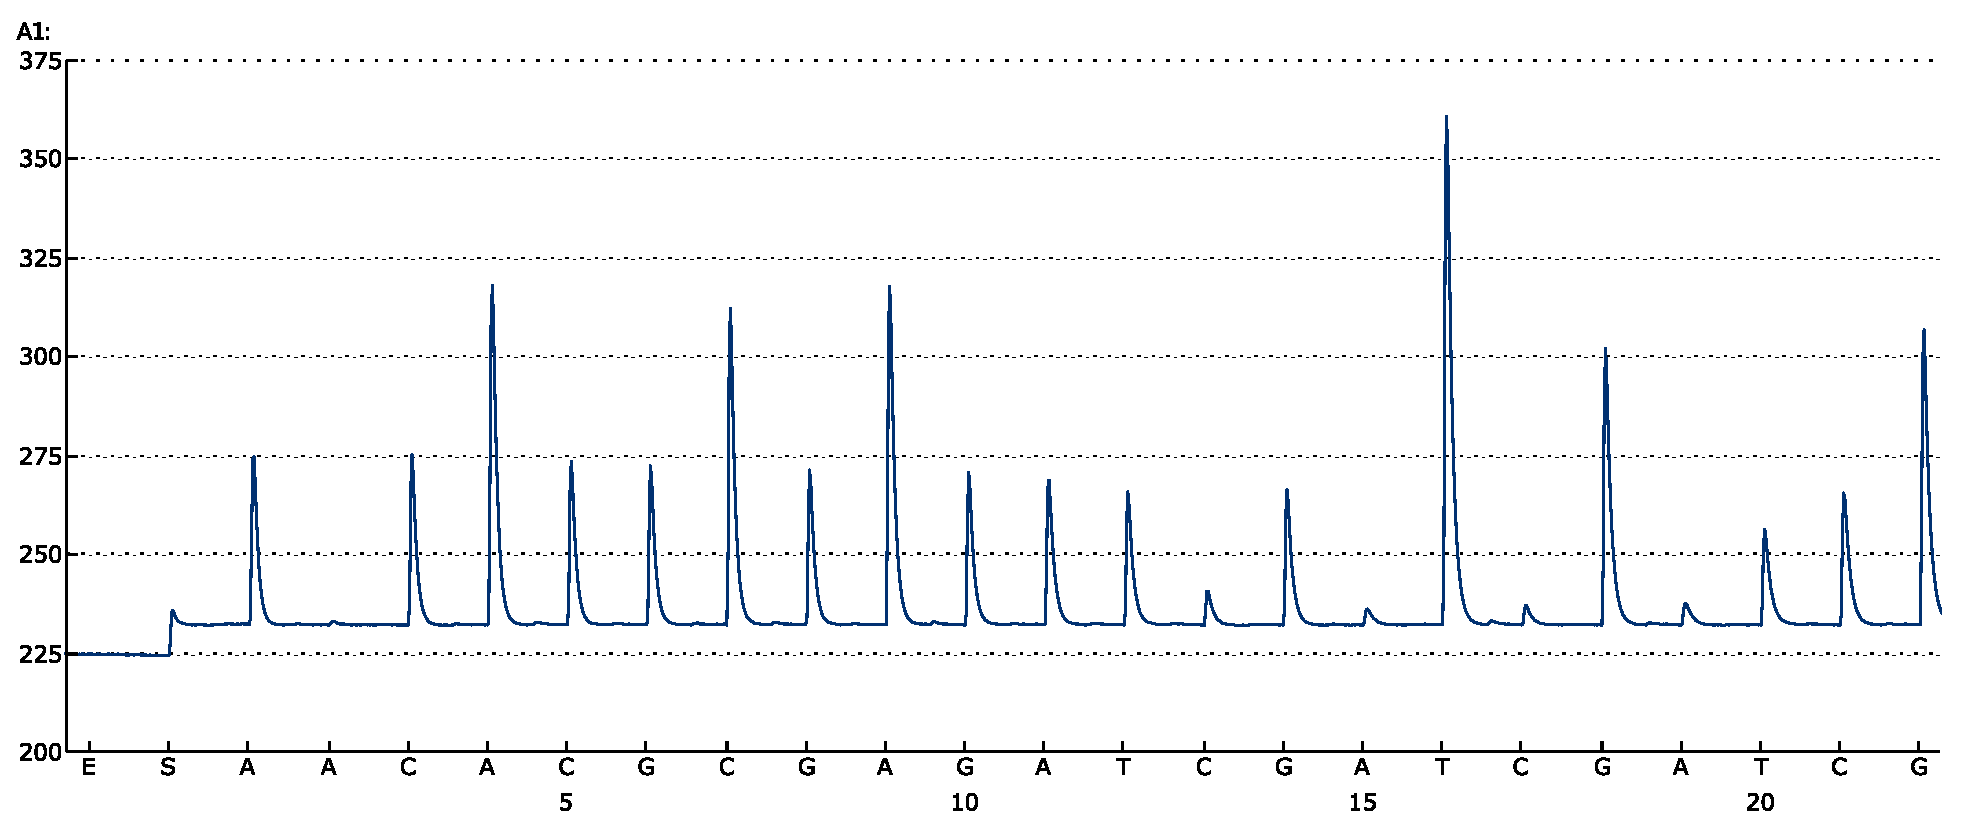
\includegraphics[width=\columnwidth]{graphics/pyrogram.eps}
      \caption{A pyrogram up to dispensation 22 (out of 104). The y-axis is
      light emittance, the x-axis is dispensation over time. When a nucleotide
      is dispensed, the light emitted peaks almost immediately when the
      reaction takes place then subsides as the reaction completes.}
      \label{fig:pyrogram}
      \end{figure}

   \section{Data and Terminology}\label{sec:data_and_terms}
      In this section, the details of the data, digital representation of said
      data, terminology, and relevant synonyms used for describing all of the
      above are explained. For consistency and simplicity, the terms that will
      be used throughout the paper are established here.

      \subsection{Data}
      A data point is an individual record or object of data to be compared
      and clustered with other individual records or objects of data. While
      this seems trivial, it is important to note that a data may be a scalar
      value, a vector of values, or any other complex representation.
      Throughout this paper, we will use the term \textbf{data point} to refer
      to individual data records or patterns.

      There are three primary biological components being analyzed--isolates,
      ITS regions, and pyroprints. For the analysis described in this paper,
      the primary data point of interest is the \textit{Isolate}. Generally,
      an isolate's genome has many genes on it, and there are particular
      ITS regions of interest--for this paper and the work done with the
      Biology department, only the 23S--5S and 16S--5S ITS regions are used.
      Computationally, we simply represent an isolate as an object
      which has a reference to a set of ITS regions. Since, in practice, a
      pyroprint is constructed by pyroprinting an ITS region of the isolate
      genome, we represent an ITS region as a collection of pyroprints. A
      Pyroprint is output from the pyrosequencer as a pyrogram of light
      emittance per nucleotide dispensation--a character in the alphabet
      \textbf{A}, \textbf{T}, \textbf{C}, or \textbf{G}. We easily represent a
      pyroprint as a vector of floating point values (light emissions) where
      each component corresponds to a dispensed nucleotide. In this way, the
      biological components and their relationships are represented in an
      object-oriented manner. More details are described in Section
      \ref{sec:design}. More formally, given a set of isolates $I$ and an
      isolate $i \in I$, a set of ITS regions $R$ such that an ITS region $r_i
      \in R$, and a dispensation sequence $D = (d_1, \ldots, d_n)$, where $d_n
      \in \{A, T, C, G\}$, a pyroprint $\bar{p_i} = (p_i1,\ldots p_in)$, where
      $p_in$ is a real number representing the light emitted during the
      pyrosequencing process of ITS region $i$ when the nucleotide $d_n$ was
      introduced on dispensation $n$.
      
      \subsection{Metrics}
      Comparison metrics are used to compare data points based on similarity
      or dissimilarity. While similarity and dissimilarity are two sides of
      the same coin, the ease of conversion between the two varies based on
      the comparison metric used. In this paper, our analyses are based on
      similarity values. This is so chosen because the comparison metric used
      for pyroprints is \textit{Pearson's Correlation}--a similarity metric
      defined in Equation \ref{eq:pearson}. Unfortunately, pyrosequencing machines
      are observe fluctuations in the amplitude of light emitted
      during binding reactions in the sequencing process. Pearson's correlation
      is ideal for accommodating these fluctuations because it is
      concerned with comparing the variance between a pair of pyroprints
      $\bar{p_x}$, $\bar{p_y}$ instead of a direct comparison between the
      values $p_xn$, $p_yn$.

      In order to appropriately interpret the computed correlation coefficient
      between a pair of pyroprints, we utilize a pair of threshold values
      $\alpha$, the \textit{upper threshold}, and $\beta$, the \textit{lower
      threshold}\footnote{Default values are $\alpha = .995$ and $\beta =
      .99$}. We use these thresholds to qualify whether the
      similarity between two pyroprints is high enough to warrant grouping
      their isolates together, or low enough to guarantee that their isolates
      should not be grouped together. Since these thresholds may vary depending
      on the ITS region and the selected FIB, each ITS region
      $r_i$ is associated with its own pair of thresholds, $\alpha_i$ and $\beta_i$.
      More specifically, if the similarity between two pyroprints is greater
      than $\alpha$ ($sim(\bar{p_1}, \bar{p_2}) > \alpha$) then the two
      pyroprints are considered the same, or identical. Conversely, if
      $sim(\bar{p_1}, \bar{p_2} \le \beta$, then the two pyroprints are
      considered \textit{definitely} different. The range between $\alpha$ and
      $\beta$ is colloquially called the \textit{squishy region} and
      similarities that fall in that range are inconclusively similar or
      dissimilar because we do not know whether it is experimental error or
      actual differences that account for the low similarity. The way this is
      handled is described in Chapters \ref{chap:algorithm} and
      \ref{chap:implementation} as appropriate.

   \section{Clustering}\label{sec:clustering}
      Cluster analysis, or clustering for short, is the organization of a
      collection of patterns, or data points, into clusters based on
      similarity~\cite{Jain:DataClustering}. Using similarity, computed by
      functions appropriately determined for comparison between patterns, the
      process of clustering is as simple as grouping patterns with the highest
      calculated similarity above some threshold parameter(s).

      Clustering is innately fuzzy, as it is commonly referred to as
      \textit{unsupervised learning}. Since the objective of clustering is to
      organize data according to relationships with minimal manual
      intervention, the definition of which data points should and shouldn't be
      grouped and is not well defined. Threshold parameters are the typical
      approach to addressing this issue in clustering. A threshold is a value
      or level that a comparison, in our case similarity, must meet--similarity
      must be above, dissimilarity must be below. In this way, the threshold
      parameter can be tuned to better suit various data sets with minimal
      intervention. Intuitively, a threshold can be described as the point at
      which two data points are believed to be highly related or even
      identical. This will have different interpretations depending on the data
      being analyzed and the objective of the analysis being carried out.
      Intuitively, if two isolates differ substantially, then the two isolates
      belong to different strains. The thresholds used for clustering are based
      on the thresholds given for each ITS region.
   
      \textbf{Data Transformation}. Hierarchical clustering algorithms, including the
      algorithm we developed here, work by comparing, on each step, groups of data
      points (pyroprints, in our applications) and combining similar data points to
      each other. Our algorithm uses a \textit{thresholded version} of the Pearson
      correlation coefficient to compare individual pyroprints to each other (see
      Equation \ref{eq:threshold}. Anytime inter-cluster similarity measures are
      calculated, our algorithm applies a threshold function (Equation
      \ref{eq:threshold}) which returns $1$ if the two pyroprints are the same, and
      $0$ if the respective pyroprints are definitely dissimilar. These cases are
      represented by the relationships $sim(\bar{X}, \bar{Y}) \ge \alpha$ and
      $sim(\bar{X}, \bar{Y}) < \beta$, respectively. Similarities between $\alpha$ and
      $\beta$ are left unmodified. This transformation is the mechanism for ensuring
      strongly connected isolates at the core of each cluster. We represent already
      constructed clusters of pyroprints using a single pyroprint vector representing
      average values of the cluster known as the \textit{average-link} hierarchical
      clustering method. Average-link inter-cluster similarity measures are
      calculated using Equation \ref{eq:cluster_sim}. In this function, $\alpha_r \in
      A$, $\beta_r \in B$ $\forall r \in R$ represents the threshold pair for each
      ITS Region $r$. $C$ is the set of clusters such that $C_m \in C$ and $\exists i
      \in I$ such that $i \in C_m$.

      \textbf{Clustering Algorithm}. Previous data sets used for analysis contained a
      large number of isolate pairs whose pyroprints had similarity between $0.995$
      and $1$. In such situations, knowing that two pyroprints collected from the
      same sample have a high similarity is sufficient to put them into a single
      cluster \textit{immediately}, even though a pyroprint from another month may
      have a higher similarity with one of them. In consideration of this, the
      algorithm we have developed constructs clusters in a two step process: (1)
      cluster all isolates that are \textit{strongly connected}\footnote{A set of
      pyroprints $P$ is considered \textit{strongly connected} if each pyroprint $p
      \in P$ is sufficiently similar (i.e. \textit{connected}) to every other
      pyroprint in $P$} in an order determined by the user; (2) cluster the remaining
      isolates with the clusters formed in step 1 using traditional hierarchical
      clustering. By integrating the remaining isolates into clusters in the last
      step, we minimize the negative effect that \textit{weakly connected} isolates
      have on cluster construction.

      The structure depicted in Appendix \ref{sec:structural_organization} dictates
      clustering order. Conceptually, this process occurs in the following manner:
      isolates located in the leaves of the structure are clustered using traditional
      hierarchical clustering. The resulting clusters are then propagated up the tree
      to the parent nodes. Optionally, the user may specify whether to incrementally
      grow clusters or to integrate all clusters together at once. This specific
      implementation of the approach incrementally grows clusters. This
      incremental growth is representative of the approximate chronology in which
      isolates were collected. This process repeats%for each swabbing technique, and
      for each month in the study until clustering of all isolates in the structure
      is complete.

\chapter{Algorithms}\label{chap:algorithm}
      Once strain similarity/dissimilarity of data points are quantified,
      hierarchical clustering methods (e.g., CLUSTAL or Primer5~\cite{Primer5:methods})
      are commonly used to analyze the obtained data and determine
      how many strains were present among the obtained bacterial isolates.
      
      If $sim(\bar{X}, \bar{Y})$ is
      sufficiently close to $1$, we assume $X$ and $Y$ come from the same strain.
      However, if $sim(\bar{X}, \bar{Y})$ is sufficiently far from $1$, then $X$ and
      $Y$ \textit{definitely come from different strains}.

      As an aggregate of several, variable copies of a DNA region, pyroprints
      are patterns of DNA which capitalize on the differences between the
      replicates of the ITS regions and serve as the basis of comparison
      between \textit{E. coli} isolates. A ``match'' between \textit{E. coli}
      isolates is determined when the pyroprints for both ITS 1 and 2 are
      considered identical between two isolates.

   \section{OHClust!}\label{sec:ohclust}
      \subsection{Algorithm}
         \begin{enumerate}
            \item create feature ontology
            \item parse data (multiple matrices or from database)
            \item organize data into feature ontology
            \item walk tree nodes and cluster where data is present (leaves)
            \item when all children of a node have been clustered, the data in the
                  node is clustered, and these clusters are returned up to the
                  parent
         \end{enumerate}

         \begin{algorithmic}
            \Function {clusterDataStructure}{$D$, $N$}
               \State $C \gets \emptyset$

               %If this node is null then return emptyset
               \If {$N = null$}
                  \Return $C$
               \EndIf

               %If this node has children then cluster them before this node
               \If {$|$children($N$)$| > 0$}
                  \For {$n_i \in$ children($N$)}
                     \State $C \gets C\ \cup$ clusterDataStructure($D$, $n_i$)

                            \If {isChronological($N$)}
                        \State $C \gets C\ \cup$ performHierarchical($D$, $C$)
                     \EndIf
                  \EndFor

                  \If {!isChronological($N$)}
                     \State $C \gets C\ \cup$ performHierarchical($D$, $C$)
                  \EndIf

               %If this is a leaf node then just cluster the data
               \Else
                  \State $C \gets$ performHierarchical($D$, $C$)
               \EndIf

               %Return clusters to parent
               \Return $C$
            \EndFunction

            \Function {performHierarchical}{$D$, $C$}
               \State $C' \gets C$
               \State ($c_a$, $c_b$) $\gets \emptyset$
               \State $S[j,k] \gets$ recomputeDistances($C'$)
               \For {$c_j$, $c_k$ $\in C'$}
                  $S[j, k] \gets$ sim($c_j$, $c_k$)
               \EndFor

               \While {$|C'| > 1$ and sim($c_a$, $c_b$) $\ge \alpha$}
                  \State ($c_a$, $c_b$) $\gets$ \textit{arg}min($S[j,k]$)
                  \If {sim($c_a$, $c_b$) $\ge \alpha$}
                     \State $C' \gets C'\ \cup$ combineClusters($c_a$, $c_b$)
                     \State $S[j,k] \gets$ recomputeDistances($C'$)
                  \EndIf
               \EndWhile

               \For {$c_i \in C$}
                  \If {$|c_i = 1$}
                     \State $W \gets W\ \cup c_i$
                  \EndIf
               \EndFor
            \EndFunction

            \Function {recomputeDistances}{$S$, $C$}
               \For {$c_j$, $c_k \in C$}
                  \If {sim($c_j$, $c_k$) $\ge \alpha$}
                     \State sim($c_j$, $c_k$) $\gets 1$
                  \ElsIf {sim($c_j$, $c_k$) $< \beta$}
                     \State sim($c_j$, $c_k$) $\gets 0$
                  \EndIf
               \EndFor

               \Return $S$
            \EndFunction
         \end{algorithmic}

\chapter{Related Work}\label{chap:related}

   \section{Incremental Clustering}\label{sec:incr_cluster}
   Since OHClust! is claimed to be applicable to data types other than
   biological, this section discusses incremental clustering algorithms
   developed for generic datasets. These algorithms were developed to
   incrementally cluster data streams or datasets too large to fit in main
   memory. While this definition of incremental clustering is still applicable
   and relevant to our notion of incremental clustering, there are some
   assumptions that may cause divergence between the optimal clustering of a
   growing dataset and proposed clustering of these algorithms. More
   specifically, clustering a dataset in increments, still has the assumptions
   of a single, whole dataset. In contrast, clustering a dataset that is
   updated in increments has the assumptions that the ideal number of clusters
   may change between updates. The subtle difference may make a difference in
   how quickly produced clusters diverge from optimal clusters, and thus affect
   how frequently the accumulated dataset must be re-clustered.

   %BIRCH description%
   BIRCH, Balanced Iterative Reducing and Clustering using Hierarchies, is a
   clustering method developed by Zhang, et al. to address the problem of
   clustering large datasets and minimizing I/O costs~\cite{Zhang:BIRCH}. BIRCH
   incrementally clusters numerical data by doing a scan of the target dataset
   until memory constraints are reached. Each chunk of data is added to an
   N-ary tree, called a cluster feature (CF) tree, which represents clusters as
   internal nodes and maintains only aggregate information for each cluster.
   The aggregate information, and clustering requirements, are computed based
   on basic algebraic functions: Each data point is represented as a triple of
   the form $D = (N, LS, SS)$ where a data point $D$ is assumed to be a vector,
   $N$ is the number of dimensions, $LS$ is the linear sum of the dimensions of
   $D$, and $SS$ is the squared sum of the dimensions of $D$. In this way,
   distances (not similarities) are additive and easily computed in a single
   scan of the data. This approach uses the CF Tree as a fast, guiding method
   for directing a data point to the appropriate cluster. However, determining
   an appropriate, meaningful CF representation is difficult at best.

   %Fast and Stable Incremental Clustering description%
   Young, et al.'s work on incremental clustering takes a 
   partitional approach to clustering~\cite{Young:Incremental}. The described
   work utilizes a competitive learning algorithm that adjusts itself based on
   a calculated pseudo-entropy of the clusters such that a
   tradeoff is made between updating centroids aggressively earlier in the
   clustering process (earlier iterations and/or updates)
   and updating centroids conservatively later to ensure cluster stability.
   Additionally, there is a credit-based algorithm for preventing centroid
   starvation which is computed based on a fixed value or the previously
   calculated pseudo-entropy such that centroids selected for updates lose
   credit and centroids that are starving accumulate credit over time. Although
   Young, et al. mention the importance of being mindful of the possibility
   that clusters may move, disappear, or reappear, the described work only
   discusses moving centroids and assumes a fixed number of centroids. Since
   the number of clusters that may be formed from clustering pyroprints is
   completely unknown, and will grow unpredictably as more data is gathered
   from different regions, a partitional scheme with a fixed number of
   centroids is not very applicable.

   \section{Incremental Clustering for 16S rRNA Sequences}\label{sec:seq_incr_cluster}
   This section discusses incremental clustering algorithms that were
   developed specifically for clustering DNA sequence reads. These are
   especially relevant to the work described in this paper as OHClust! was
   developed with pyroprints in mind. Incremental clustering algorithms
   described in this section are all derived from a greedy incremental sequence
   clustering algorithm, hereafter referred to as \textit{SeqClustering} for
   brevity, developed in 1998 by Holm and Sander~\cite{Holm:Greedy}. The
   motivation for this incremental clustering algorithm was to effectively
   handle continuously growing biological datasets, specifically protein
   sequences, and to efficiently determine and convey clusters of similar
   protein sequences. Due to the high volume of redundant protein sequence
   reads, Holm and Sander decided that each cluster should be represented by a
   single data point, or sequence read. By using a representative data point
   for each cluster, it was much more efficient to compute cluster membership
   for each unclustered data point and to convey meaningful, non-redundant
   information for understanding each cluster. Variants of this clustering
   algorithm refer to the representative sequence read of a cluster as a
   \textit{seed}. This algorithm, as well as its variants such as
   CD-HIT~\cite{Li:CD_Hit}, UCLUST~\cite{Edgar:UCLUST}, and
   DySC~\cite{Zheng:DySC}, cluster DNA sequences by using a single sequence as
   a cluster representative to which unclustered DNA sequences are aligned
   against. That is, DNA sequences are data points, and each cluster is
   represented by a single data point, against which other data points are
   compared. The comparison metric used is typically a sequence alignment,
   which gives a similarity score based on the edit distance between the
   compared sequences.

   One variant of Holm and Sander's SeqClustering algorithm is cd-hit and each
   of its variants: cd-hit-2d, cd-hit-est, cd-hit-est-2d~\cite{Li:CD_Hit,
   Li:Redundancy}. Cd-hit has SeqClustering as its core algorithm, but
   optimizes performance by using short word filtering instead of sequence
   alignments as its comparison metric. Short word filtering, in short,
   verifies that the compared sequences share a minimum number of identical
   short substrings, referred to as `words', such as dipeptides, tripeptides,
   etc. For certain length words, it's possible to have indices of the seed for
   a cluster so that it is very fast to compare a sequence to the seed via
   short word filtering.

   %DySC Greedy Clustering Description%
   Another, very relevant, variant of the SeqClustering algorithm, called
   dynamic seed clustering (DySC), was developed by Zheng, et
   al.~\cite{Zheng:DySC}. DySC is a clustering algorithm developed for reads of
   the 16S rRNA marker gene commonly used in microbial studies.  DySC
   differentiates itself from other SeqClustering algorithms by using both
   fixed seeds and dynamic seeds. Seeds in SeqClustering correspond to a fixed
   seed in DySC, whereas SeqClustering has no equivalent to dynamic seeds in
   DySC. Using dynamic seeds, DySC constructs \textit{pending clusters},
   clusters containing reads that are not within a similarity threshold to the
   fixed seeds. Pending clusters are transient and will either join a fixed
   seed cluster or become a fixed seed cluster after reaching a specified size.
   Zheng, et al. claim that DySC is able to improve cluster quality while
   maintaining comparable runtime compared to UCLUST and
   CD-HIT~\cite{Zheng:DySC}.

   %Incremental Clustering Description%
   Yooseph, et al. have done work on the incremental clustering of microbial
   metagenomic sequence data~\cite{Yooseph:Incremental}. Incremental clustering
   is a three stage clustering process based on CD-HIT. \textbf{First Stage}.
   patterns are combined with clusters in three steps, each with 90\%, 75\%,
   and 60\% identity thresholds, respectively. Incremental clustering takes
   this approach of decreasing identity thresholds for efficiency and quality.
   For efficiency, cd-hit-2d runs faster at high thresholds (90\%) than at low
   thresholds (60\%). For quality, the parallel implementation of cd-hit-2d
   being used by Yooseph, et al. at the time (2008) could only assign patterns
   to the first cluster whose similarity met the threshold. \textbf{Second
   Stage}. Patterns from the data set not incorporated into clusters in stage
   one are clustered together using cd-hit at 90\%, 75\%, and 60\% identity.
   The clusters formed here are referred to as \textit{core clusters} by
   Yooseph, et al. \textbf{Third Stage}. Two similarity measures are used to
   join \textit{big core clusters} (cluster with cardinality $\ge$ 20) with
   each other and small core clusters or singleton clusters (cluster with
   cardinality $=$ 1) with final clusters, respectively FFAS and PSI-BLAST.
   
   %Relate algorithms to work%
   Each variant of the SeqClustering algorithm is highly relevant to OHClust!
   in their ability to cluster data incrementally and their relevance to
   biological data. Using a seed, or cluster representative, that is $\le 90\%$
   similar to all other seeds allows new clusters to easily form, which is
   important to consider for a continuously growing dataset. Interestingly,
   Yooseph, et al.'s work on incremental clustering and its three phase
   approach seems to be the most similar to OHClust!. Where Yooseph, et al.
   takes a three phase approach, OHClust! seeks to improve clustering
   performance and quality in a two phase approach. The first phase creates
   core clusters using the $\alpha$ threshold, and the second phase
   incorporates pyroprints into a boundary or fuzzy cluster using the $\beta$
   threshold. However, incremental clustering partitions its data in a three
   tier scheme by thresholds (90\%, 75\%, and 60\%) instead of the hierarchical
   partitioning employed by OHClust!.
   
   Seemingly, these algorithms are more accommodating of updates than
   incremental clustering in Section \ref{sec:incr_cluster} and can handle
   situations where constructed clusters may significantly differ from initial
   predictions of observable patterns. In this way, these algorithms may be
   more amenable to incremental clustering across updates than OHClust!.
   However, there is a major aspect in which SeqClustering algorithms differ
   from OHClust!: the use of a core cluster in OHClust! instead of a
   representative data point. Instead of a representative data point, the use
   of core clusters potentially reduces clustering errors of pyroprints,
   especially across updates. This is especially important since pyroprints are
   not exactly DNA sequences and are vulnerable to machine and human error.
   Additionally, cluster similarity is computed using each point in the cluster
   (in the case of average-link or ward's method) instead of a single
   comparison. Due to this being computationally more expensive, the advantages
   and disadvantages of not using cluster representatives are explored in
   Chapter \ref{chap:evaluation}.

   %Temporal clustering, as described by Kamath and
   %Caverlee~\cite{Kamath:Transient}, is a variation of clustering that models
   %data as a communication network. Nodes represent members in the
   %communication network while edge weights represent communication between
   %said nodes. The edge weights in the network are based on when the messages
   %are exchanged. Kamath and Caverlee utilize 3 different edge weight decay
   %functions to reflect temporal locality. Their naive function decrements edge
   %weights by 1 between two nodes where a message was not exchanged by the two
   %nodes during a specific time interval. Otherwise the edge weight is
   %incremented by 1. Another suggested decay function, \textit{fixed window},
   %only utilizes edge weights where communication occured during a time window
   %$\beta$. Edge weights are ignored if communication between two nodes occurs
   %outside of this time window. The final edge weight decay function proposed,
   %\textit{exponential decay}, is the final function proposed in
   %\cite{Kamath:Transient} and was the chosen function used in Kamath and
   %Caverlee's temporal clustering. This uses a parameter $\xi$ that is used to
   %identify crowds gathering at relative rates. A higher $\xi$ is used for
   %identifying crowds which form quickly and a lower $\xi$ identifies crowds
   %forming slowly. More formally:
   %\textit{Messages not exchanged:}
      %\begin{description}
         %\item w$_{t}$(u, v) = w$_{t - 1}$(u, v) - log(T$_{now}$ - $\tau$(u, v))
               %$\times$  $\xi$ 
      %\end{description}

   %\textit{Messages exchanged:}
      %\begin{description}
         %\item w$_{t}$(u, v) = w$_{t - 1}$(u, v) + 1 - log(T$_{now}$ - $\tau$(u, v))
               %$\times$  $\xi$ 
      %\end{description}
   %$\tau$(u, v) is the time of the last communication between nodes u and v. This
   %way the longer the gap in communication between two nodes, the lower the edge
   %weight connecting the two nodes.

   %Qamra, Tseng, and Chang~\cite{Qamra:BlogMining} suggest a \textit{modified
   %time-sensitive dirichlet process model} based on work by Jhu, et
   %al.~\cite{Jhu:Dirichlet}. This clustering algorithm is similar to the
   %Chinese Restaurant Process but also incorporates
   %time~\cite{Qamra:BlogMining}. The probability of joining a group (cluster) depends on the
   %group members and their respective ages. There is also some probability,
   %determined by a \textit{concentration parameter}, that a new cluster will be
   %formed. As group members age, their respective influence in the group decays.
   %The time-sensitive dirichlet discussed by Jhu, et al.~\cite{Jhu:Dirichlet}
   %was modified by Qamra, et al. to calculate a uniform probability of being
   %assigned a new cluster. The decay of a blog story's influence in a cluster
   %is controlled by a kernel function so that new entries are less likely to
   %join older stories.

   %\textit{PoClustering} (partially ordered clustering) clusters data into
   %\textit{PoSets} (partially ordered sets) by finding all clique clusters for
   %all possible diameters W(D) where D is the maximal dissimilarity in a
   %dissimilarity matrix~\cite{Liu:CPD}. PoClustering is a generalization of both
   %hierarchical and pyramidal clustering that allows overlaps between clusters such that a
   %PoCluster P is defined as P = \{cliqueset $_{\delta}$ (d) $\mid$ $\forall$ d $\in$
   %W(D)\}~\cite{Liu:PoClustering}. This ensures that PoClusters contain every
   %possible cluster with largest dissimilarity d. Additionally, hierarchical
   %and pyramidal clustering produce clusters that are subsets (special cases) of
   %PoClusters. PoClusters can be represented as a directed acyclic graph, with
   %each node representing a clique cluster and its diameter, and each edge
   %representing subset relationships between nodes. PoClusters are able to
   %successfully preserve the majority of relationships present in the data
   %whereas hierarchical clustering is unable to do so.

   %Temporal clustering and time-sensitive dirichlet modify similarity measures
   %in context of the temporal locality of particular events of interest. This
   %is slightly different from the method we propose in this paper, as we do not
   %modify similarity measures of \textit{E. coli} isolates based on
   %chronological distance. Instead, we simply enforce a particular ordering on
   %cluster candidates based on a given, defined ontological structure. 
   %Similarly, PoClustering enforces a particular ordering on the clustering
   %process without modifying similarity measures. Although PoClustering is not
   %time-sensitive, it is important related work for our method regarding
   %connectivity constraints between \textit{E. coli} isolates.

   %TODO
\chapter{Implementation}\label{chap:implementation}
   %The implementation described in this chapter was done in Java, and compliant
   %with Java 1.6 since the majority of users have Java 1.6 installed, not Java
   %1.7. Additionally, the code is accessible from the SPAM repository on my
   %GitHub account\footnote{http://www.github.com/drin/spam}. This chapter also
   %has a dual purpose of describing how the algorithm has been implemented, and
   %providing a reference of documention for anyone desiring to use or extend
   %the code provided.

   \section{SPAM - Suite of Pyroprint Analysis Methods}\label{sec:spam}
      This section discusses the implementation of the framework
      \textit{SPAM}--Suite of Pyroprint Analysis Methods. This framework is
      written such that many components can be written consistently and
      interchangeably, including clustering methods, comparison metrics, and
      data types. In Section \ref{sec:design} the overall design of
      the framework is described, while Sections \ref{sec:data_types} and \ref{sec:metrics}
      discuss how data types can be written, and how comparison metrics are
      called and can be implemented, respectively. Finally, Section
      \ref{sec:analysis} details how analysis methods--particularly
      hierarchical clustering methods--can be extended and customized.

      \subsection{Design}\label{sec:design}
         The framework was designed to be modular. Particularly, it was desired
         that it would be easy to swap comparison metrics and clustering
         methods. In order to do this, an abstract approach for defining and
         using various data types had to be designed.
         
         The basic design is that custom data types extend a
         \textit{Clusterable} abstract class interface.


         However, to ensure a flexible and
         maintainable system, isolates are represented as a complex data point
         that is associated with \textit{ITS Regions} and \textit{Pyroprints}.

      \subsection{Data Types}\label{sec:data_types}

      \subsection{Comparison Metrics}\label{sec:metrics}

      \subsection{Analysis Methods}\label{sec:analysis}

\chapter{Evaluation}\label{chap:evaluation}
   For evaluation of OHClust!, resulting clusters are compared against the
   clusters of \textit{Agglomerative Hierarchical
   Clustering}--\textit{HClustering} for short. Given the wide use of
   HClustering by biologists on biological datasets, HClustering is used as
   the baseline to compare OHClust! against. Preliminary results on the
   comparison of accuracy was done in a previous case
   study~\cite{Montana:ChronoCluster}, but, in this section, the
   clusters produced by the two algorithms are compared more thoroughly, on larger, more
   complex datasets, and both algorithms are analyzed for their performance. In many
   cases, OHClust! is expected to produce clusters $C$ that are a
   \textit{refinement} of clusters from HClustering, $C'$. That is, each
   cluster $C_i \in C$ is contained in a cluster of $C'_k \in C'$,
   formally\footnote{This definition of refined clusters comes from
   Wagner~\cite{Wagner:Overview}}:
   $$\forall C_i \in C, \exists C'_k \in C' : C_i \subseteq C'_k$$.
   Below, both the hypothesis and evaluation plan are described before discussing
   results in Section \ref{sec:results} and relevant conclusions in Section
   \ref{sec:conclusion}.

   \section{Hypothesis}\label{sec:eval_goals}
      For the comparison between OHClust! and HClustering, the resulting
      clusters of both algorithms are expected to be largely similar. This is
      formalized by the null hypothesis $H_0: VI(C, C')$ is very close to $2/n$
      (Not yet actually determined). $VI(C, C')$ is the variation of
      information~\cite{Halkidi:Validation} between the set of OHClust!
      clusters $C$ and the set of HClustering clusters $C'$ defined as:
      $$VI(C, C') = H(C) + H(C') - 2I(C, C')$$
      where:
      $$P(i) = \frac{C_i}{n}$$
      $$P(i,j) = \frac{| C_i \cap C_j'}{n}$$
      $$H(C) = -\sum_{i=1}^{k}P(i)log_2P(i)$$
      and
      $$I(C, C') = \sum_{i=1}^{k}\sum_{j=1}^{t}P(i,j)log_2\frac{P(i,j)}{P(i)P(j)}$$
      In the above equations, $n$ is the number of clusters, $P(i)$ is the
      probability that an element $x$, at random, is in the cluster $C_i \in C$
      and $P(i, j)$ is the probability that an element $x$ is in the clusters
      $C_i \in C$ and $C'_j \in C'$, where $|C_i \cap C'_j|$ is the size of the
      intersection between clusters $C_i$ and $C'_j$. shannon's entropy,
      $H(C)$, can then be calculated for $C$ and $C'$. Relating the entropy of
      both sets of clusters, $H(C)$ and $H(C')$, we then calculate the mutual
      information between $C$ and $C'$, $I(C, C')$.

      Additionally, it is expected that while the performance of OHClust! and
      HClustering should be relatively similar for a given raw dataset,
      OHClust! will perform much faster than HClustering when given additional
      data, that still fits the ontology specified, to be clustered. This
      expectation is based on the ability of OHClust! to analyze and
      incorporate clusters in newly collected data with clusters previously
      formed, whereas HClustering may incorrectly join new data to previously
      constructed clusters, and thus must completely re-analyze the entire
      dataset when new data is introduced.

   \section{Evaluation Plan}\label{sec:eval_plan}
      The evaluation plan detailed in this section focuses on the question
      ``how does the performance of OHClust! compare to HClustering?'' while at
      the same time ensuring that \textit{The clusters formed by OHClust! and
      HClustering do not diverge significantly.} The divergence between
      HClustering and OHClust! is important to consider since there is no clear idea
      of what resulting clusters \textbf{should} look like, so by showing that
      the clusters formed by each algorithm are similar enough to each other,
      it can be seen that OHClust! is no less accurate than HClustering, and
      thus, accuracy is not an issue.

      My evaluation plan is motivated by the following evaluation goals:
      \begin{itemize}
         \item Show that the clusters formed by OHClust! are insignificantly
               dissimilar from HClustering.
         \item Determine how many data points may be added before the
               dissimilarity between OHClust! and HClustering clusters
               significantly diverge.
         \item Assess the performance benefits of using OHClust! in a
               microbial source tracking system in place of HClustering. More
               specifically:
               \begin{itemize}
                  \item On average, how much time is saved using OHClust!?
                  \item In the worst case, where OHClust! must re-analyze the
                        entire dataset, what is the performance difference
                        between OHClust! and Hierarchical Agglomerative?
               \end{itemize}
      \end{itemize}

      The test harness for SPAM consists of three parameters: a configuration,
      a clusterer, and a data set. The configuration is a java class that
      contains all of the parameters needed by any clusterer. These
      parameters are all of the variables that we need to alter during our
      evaluation tests in order to fully characterize the analysis methods and
      their applicability:
      \begin{itemize}
         \item Similarity thresholds(i.e. $\alpha$ and $\beta$):
               \begin{itemize}
                  \item ITS Region
                  \item Cluster
               \end{itemize}
         \item Similarity transformations in relation to isolate similarity
               thresholds
         \item Pyroprint dispensation lengths (per ITS region)
         \item Inter-cluster and inter-ITS region distance metrics:
               \begin{itemize}
                  \item Single-link
                  \item Complete-link
                  \item Average-link
               \end{itemize}
      \end{itemize}
      Some properties of the two algorithms that should be observed:
      \begin{itemize}
         \item Compactness--members within a cluster should be as similar, or
               close, as possible.
         \item Separation--clusters should be as separated, or dissimilar, as
               possible.
      \end{itemize}

      (This is written as if the tests are already done) While there are many
      parameters that can be tuned to characterize the behaviors of OHClust!,
      It is unnecessary to compare the results from all configurations of
      OHClust! with all configurations of HClustering. The tests that have been
      ran include several configurations of OHClust! compared against each other, and the
      comparison of one configuration of HClustering to the same configuration
      of OHClust!. The different configurations of OHClust! that were tested
      can be seen in Figure \ref{tab:ohclust_configs}.

      \begin{table}[t]
      \centering
      {\small
      \begin{tabular} {| c | c | c | c | c | c | c | c | c |}
      \hline
         \textbf{T} & \textbf{Num Itrs} & \textbf{Itr Incr} & \multicolumn{2}{| c |}{\bf Metrics} \\
      \hline
                    &                   &                   & inter-cluster & inter-ITS     \\
      \hline                           
         Yes        & 50                & 50                & average-link  & average-link  \\
      \hline                                               
         No         & 50                & 50                & average-link  & average-link  \\
      \hline                                               
         Yes        & 100               & 25                & average-link  & average-link  \\
      \hline                                               
         No         & 100               & 25                & average-link  & average-link  \\
      \hline                                               
         Yes        & 100               & 50                & average-link  & average-link  \\
      \hline                                               
         No         & 100               & 50                & average-link  & average-link  \\
      \hline                                               
         No         & 100               & 50                & average-link  & average-link  \\
      \hline                                               
         No         & 100               & 50                & single-link   & average-link  \\
      \hline                                               
         No         & 100               & 50                & complete-link & average-link  \\
      \hline                                               
         No         & 50                & 50                & average-link  & median-link   \\
      \hline                                               
         No         & 50                & 50                & average-link  & complete-link \\
      \hline
      \end{tabular}
      }
      \caption{\textbf{OHClust! Test Configurations}. \textbf{Num Itrs}
               represents the number of iterations in which additional data is
               added to be clustered. \textbf{Itr Incr} represents the amount
               of data points added on each iteration. \textbf{T} represents
               whether similarities above $\alpha$ and below $\beta$ are
               transformed to $1$ and $0$ respectively. The listed metrics are
               for inter-cluster distance and inter-ITS region distance. These
               ones are listed in particular as they have the most influence on
               whether two clusters or data points will have a high similarity.}
      \label{tab:ohclust_configs}
      \end{table}


   \section{Results}\label{sec:results}
   %%%%%%%%%%%%%%%%%%%%%%%%%%%%%%%%%%%%%%%%%%%%%%%%%%%%%%%%%%%%%%%%%%%%%%%%%%%%%%%
   %%%%%%%%%%%%%% ------------- End main chapters ---------------------- %%%%%%%%%
   %%%%%%%%%%%%%%%%%%%%%%%%%%%%%%%%%%%%%%%%%%%%%%%%%%%%%%%%%%%%%%%%%%%%%%%%%%%%%%%

   %%%%%%%%%%%%%%%%%%%%%%%%%%%%%%%%%%%%%%%%%%%%%%%%%%%%%%%%%%%%%%%%%%%%%%%%%%%%%%%
   %%%%%%%%%%%%%% ------------- Begin appendices ----------------------- %%%%%%%%%
   %%%%%%%%%%%%%%%%%%%%%%%%%%%%%%%%%%%%%%%%%%%%%%%%%%%%%%%%%%%%%%%%%%%%%%%%%%%%%%%

   \section{Conclusion}\label{sec:conclusion}

\appendix

\chapter{Definitions}\label{app:definitions}
   \section{Structural Organization}\label{sec:structural_organization}
      In general, the hierarchical tree is represented as a general n-ary tree as seen in Figure
      \ref{fig:general_structure}. The parts of the tree are described as follows:
      (node) Any item in the tree, depicted as circles in Figure
      \ref{fig:general_structure}, (root) First node in the tree, located at the top,
      (leaf) A bottom-most node in the tree, (edge) A connection between any two
      nodes, (parent) In a pair of nodes with a direct connection, the parent node is
      the top node, or is closer to the root, (child) In a pair of nodes with a
      direct connection, the child node is the bottom node, or is further from the
      root, (depth) The number of edges to get from the root to a particular node,
      (level) Set of all nodes with the same depth.
      %\begin{description}
      %   \item[\em{node}] Any item in the tree, depicted as circles in Figure
      %   \ref{fig:general_structure}.
      %   \item[\em{root}] First node in the tree, located at the top.
      %   \item[\em{leaf}] A bottom-most node in the tree.
      %   \item[\em{edge}] A connection between any two nodes.
      %   \item[\em{parent}] In a pair of nodes with a direct connection, the parent
      %   node is the top node, or is closer to the root.
      %   \item[\em{child}] In a pair of nodes with a direct connection, the child
      %   node is the bottom node, or is further from the root.
      %   \item[\em{depth}] The number of edges to get from the root to a particular 
      %   node.
      %   \item[\em{level}] Set of all nodes with the same depth.
      %\end{description}

   \section{Definitions}\label{sec:definitions}
      %\begin{itemize}
      Let $I$ be the set of all isolates. Let $R$ be the set of ITS regions
      associated with $i$ $\forall i \in I$ $R$. Let $A$ be the set of all upper
      thresholds, and $B$ be the set of all lower thresholds. $\forall r \in R$,
      $\forall \alpha \in A$, $\forall \beta \in B$ let $\alpha_r$, $\beta_r$ be the
      upper and lower threshold pair corresponding to the region $r$ such that
      $\alpha_r > \beta_r$. Let $P$ be the set of all pyroprints. $\forall i \in I$,
      $\forall r \in R$ let $P_{ir} \in P$ be the pyroprint corresponding to isolate
      $i$ at ITS region $r$. Let $M$ be the set of all similaritiy matrices.
      $\forall r \in R$ let $M_r \in M$ be the matrix containing all pairwise Pearson
      correlations such that $\forall i,j \in I \times I$ $M_r[i,j] = sim(P_{ir},
      P_{jr})$
      %\end{itemize}

      \begin{figure}[H]
      \centering
      \subfloat[General]{\label{fig:general_structure}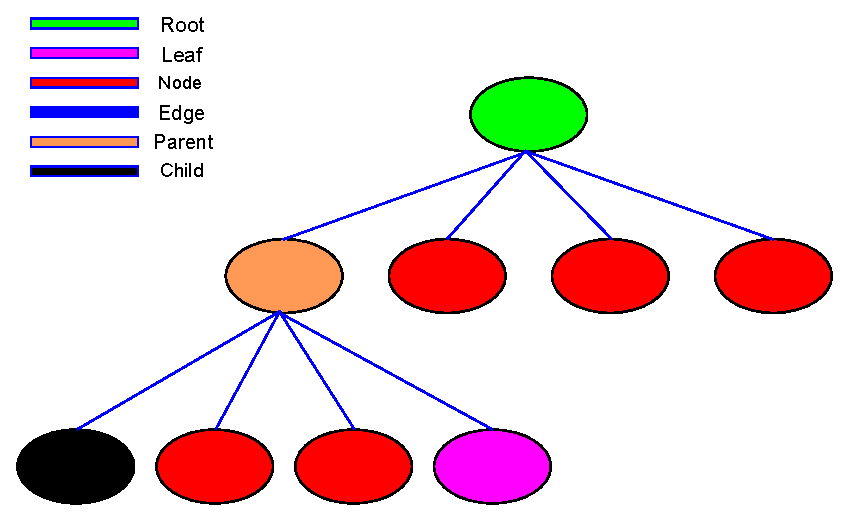
\includegraphics[width=0.5\textwidth,height=12em]{graphics/IsolateTree.eps}}
      \subfloat[Experimental]{\label{fig:cluster_structure}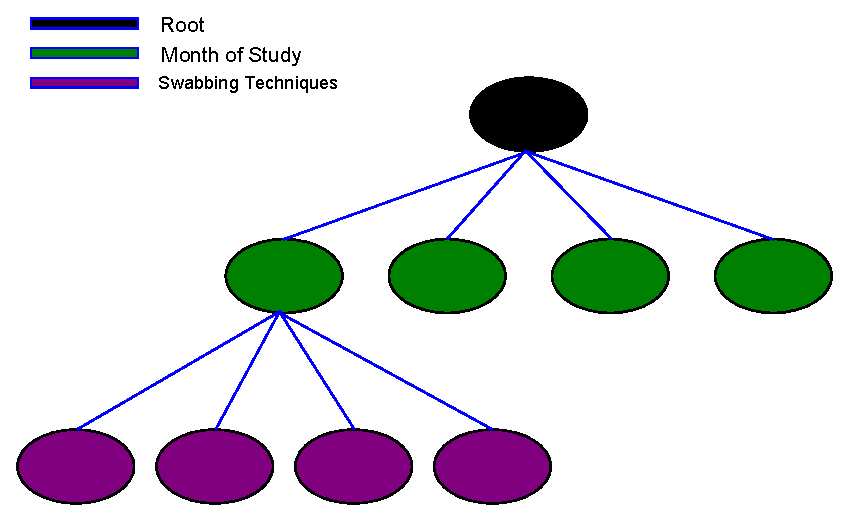
\includegraphics[width=0.5\textwidth,height=12em]{graphics/IsolateTree_CurrentStudy.eps}}
      \caption{Isolate Tree - Structural Organization: The general structure
      illustrates the parts of the organizational structure, whereas the experimental
      structure represents the month that the isolates were
      collected in the first level and the swabbing technique used to collect the
      isolate in the second level.}
      \end{figure}

   \section{Equations}\label{sec:equations}
      \begin{equation}\label{eq:pearson}
         sim(\bar{X},\bar{Y}) = \frac{\sum_{i=1}^{N}(x_i - E(\bar{X}))(y_i - E(\bar{Y}))}
         {\sqrt{\sum_{i=1}^{N}(x_i-E(\bar{X}))}\sqrt{\sum_{i=1}^{N}(y_i-E(\bar{Y}))}},
      \end{equation}
      \begin{equation}\label{eq:cluster_sim}
         sim(C_m, C_n) = i,j \in C_m \times C_n, \frac{\sum_{\forall r \in
         R}M_r[i,j]} {|C_m \times C_n|}
      \end{equation}
      \begin{equation}\label{eq:threshold}
         thr(sim(C_m, C_n)) = \begin{cases}
                              0 & if sim(C_m, C_n) < \beta_r \\
                              1 & if sim(C_m, C_n) > \alpha_r \\
                              sim(C_m, C_n) & otherwise \\
                              \end{cases}
      \end{equation}

\clearpage
\bibliography{bibliography}
\bibliographystyle{plain}
%\addcontentsline{toc}{chapter}{Bibliography}

\end{document}

%\begin{tabular} {| c | c | c | c | c | c | c | c | c |}
%\hline
   %{\bf T}          & \multicolumn{2}{| c |}{\bf Length}     & \multicolumn{4}{| c |}{\bf R}                                                     & \multicolumn{2}{| c |}{\bf Metrics} \\
%\hline
                        %& 16S--23S    & 23S--5S              & $\alpha$ (16S)      & $\beta$ (16S)      & $\alpha$ (23S)     & $\beta$ (23S)     & inter-cluster & inter-ITS     \\
%\hline                                                                                                                                                                          
   %Yes                  & 93          & 93                   & $99.5$              & $99.0$             & $99.5$             & $99.0$            & average-link  & average-link  \\
%\hline                                                                                                                                                                          
   %No                   & 93          & 93                   & $99.5$              & $99.0$             & $99.5$             & $99.0$            & average-link  & average-link  \\
%\hline                                                                                                                                                                          
   %No                   & 92          & 92                   & $99.5$              & $99.0$             & $99.5$             & $99.0$            & average-link  & average-link  \\
%\hline                                                                                                                                                                          
   %No                   & 91          & 91                   & $99.5$              & $99.0$             & $99.5$             & $99.0$            & average-link  & average-link  \\
%\hline                                                                                                                                                                          
   %No                   & 90          & 90                   & $99.5$              & $99.0$             & $99.5$             & $99.0$            & average-link  & average-link  \\
%\hline                                                                                                                                                                          
   %No                   & 93          & 93                   & $99.5$              & $99.0$             & $99.5$             & $99.0$            & single-link   & average-link  \\
%\hline                                                                                                                                                                          
   %No                   & 93          & 93                   & $99.5$              & $99.0$             & $99.5$             & $99.0$            & complete-link & average-link  \\
%\hline                                                                                                                                                                          
   %No                   & 93          & 93                   & $99.5$              & $99.0$             & $99.5$             & $99.0$            & average-link  & median-link   \\
%\hline
   %No                   & 93          & 93                   & $99.5$              & $99.0$             & $99.5$             & $99.0$            & average-link  & complete-link \\
%\hline
%\end{tabular}
%\caption{\textbf{OHClust! Test Configurations}. Each row is a different
         %configuration of an OHClust! test run. The \textbf{T} column
         %represents whether similarities above $\alpha$ and below $\beta$
         %in an ITS region are transformed to $1$ and $0$ respectively.
         %The \textbf{Length} column represents the number of
         %dispensations used for each ITS region. The \textbf{R} column
         %represents the set of $\alpha$ and $\beta$ thresholds for each
         %ITS region starting with 16S or 23S.}
